% Copyright (C) 2010,2011,2012,2013,2014 The ESPResSo project
% Copyright (C) 2002,2003,2004,2005,2006,2007,2008,2009,2010 
%   Max-Planck-Institute for Polymer Research, Theory Group
%  
% This file is part of ESPResSo.
%   
% ESPResSo is free software: you can redistribute it and/or modify it
% under the terms of the GNU General Public License as published by the
% Free Software Foundation, either version 3 of the License, or (at your
% option) any later version.
%  
% ESPResSo is distributed in the hope that it will be useful, but
% WITHOUT ANY WARRANTY; without even the implied warranty of
% MERCHANTABILITY or FITNESS FOR A PARTICULAR PURPOSE.  See the GNU
% General Public License for more details.
%  
% You should have received a copy of the GNU General Public License
% along with this program.  If not, see <http://www.gnu.org/licenses/>.
%
\documentclass[
a4paper,                        % paper size
11pt,                           % font size
twoside,                        % two sided
footsepline,                    % add a line to separate the footer
headsepline,                    % add a line to separate the header
headexclude,                    % header does not belong to the text
footexclude,                    % footer does not belong to the text
pagesize,                       % set the pagesize in a DVI document
]{scrartcl}

% Copyright (C) 2010,2011,2012 The ESPResSo project
% Copyright (C) 2002,2003,2004,2005,2006,2007,2008,2009,2010
%  Max-Planck-Institute for Polymer Research, Theory Group
%  
% This file is part of ESPResSo.
%   
% ESPResSo is free software: you can redistribute it and/or modify it
% under the terms of the GNU General Public License as published by the
% Free Software Foundation, either version 3 of the License, or (at your
% option) any later version.
%  
% ESPResSo is distributed in the hope that it will be useful, but
% WITHOUT ANY WARRANTY; without even the implied warranty of
% MERCHANTABILITY or FITNESS FOR A PARTICULAR PURPOSE.  See the GNU
% General Public License for more details.
%  
% You should have received a copy of the GNU General Public License
% along with this program.  If not, see <http://www.gnu.org/licenses/>.
%
\usepackage[draft]{varioref}    % defines \vref
\usepackage{hyperref}           % automatically creates links when
                                % using pdflatex, defines \url
\usepackage{ifpdf}              % defines \ifpdf
\usepackage{graphicx}           % handles graphics
\usepackage{color}              % use colors

\usepackage{amsmath}

\usepackage{verbatim}           % required for \verbatim and \endverbatim
\usepackage{fancyvrb}
\usepackage{calc}               % compute length
\usepackage{ifthen}             % provide ifthen
\usepackage{xspace}
\usepackage{units}
\usepackage[numbers]{natbib}

% For building the distribution docs, disable todo boxes.
%\usepackage[disable]{todonotes}
\usepackage{todonotes}

\newcommand{\es}{\mbox{\textsf{ESPResSo}}\xspace}
\newcommand{\ie}{\textit{i.e.}\xspace}
\newcommand{\eg}{\textit{e.g.}\xspace}
\newcommand{\etal}{\textit{et al.}\xspace}

\newcommand{\codebox}[1]%
{\texttt{#1}}

\DefineVerbatimEnvironment{code}{Verbatim}%
{commandchars=\\\{\}}
\makeatletter
\newenvironment{tclcode}
{%
  \addtolength{\linewidth}{-2em}% set the line length
  \@minipagetrue%%%DPC%%%
  \@tempswatrue%%%DPC%%%
  \hsize=\linewidth%
  \setbox0=\vbox\bgroup\verbatim
}{\endverbatim
  \unskip\setbox0=\lastbox%%%DPC%%%
  \egroup
  \par%
  \noindent\hspace{1em}%
  \codebox{\box0}%
  \par\noindent%
}
\makeatother

% \newcommand{\todo}[1]{
%   \marginpar{%
%     \setlength{\fboxrule}{1pt}
%     \fcolorbox{red}{yellow}{%
%       \parbox{\marginparwidth-2\fboxrule-2\fboxsep}{%
%         \bf\raggedright\scriptsize #1%
%       }%
%     }%
%   }%
% }

\makeatletter
\renewcommand{\minisec}[1]{\@afterindentfalse \vskip 1.5ex
  {\parindent \z@
    \raggedsection\normalfont\sffamily\itshape\nobreak#1\par\nobreak}%
  \@afterheading}
\makeatother

\newcommand{\esptitlehead}{
  \titlehead{
    \begin{center}
      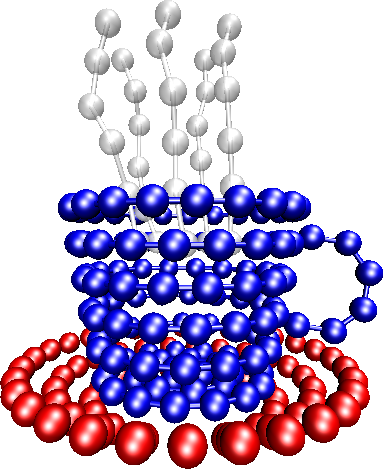
\includegraphics[width=5cm]{logo/transparentbg}
    \end{center}
  }
}

\usepackage[export]{adjustbox}

\begin{document}
\esptitlehead
\title{Tutorial: Object in fluid
\ifdefined\esversion
\thanks{For \es \esversion}
\fi
}

\maketitle
\tableofcontents

\section{Introduction}

This tutorial introduces some of the features of \es module Object in fluid (OIF). Even though \es was not primarily intended to work with closed objects, it appears very suitable when one wants to model closed objects with elastic properties, especially if they are immersed in a moving fluid. Here we offer a step by step Tcl tutorial that will show you how to use this module. The resulting code can be run using \verb|Espresso <file>| from the \es source directory. It produces .vtk files that can then be visualized using Paraview.\\

The OIF module was developed for simulations of red blood cells flowing through microfluidic devices and therefore the elasticity features were designed with this application in mind. However, they are completely tunable and can be modified easily to allow the user model any elastic object moving in fluid flow.  

\begin{figure}[htbp]
  \hfill
  \begin{minipage}[t]{.32\textwidth}

      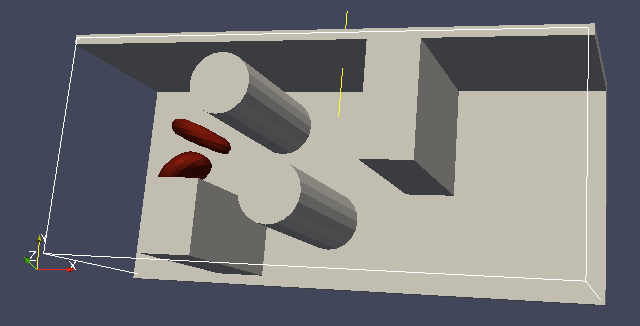
\includegraphics[width=4.3cm,right]{figures/1.png}

  \end{minipage}
  \hfill
  \begin{minipage}[t]{.32\textwidth}
   \begin{center}  
      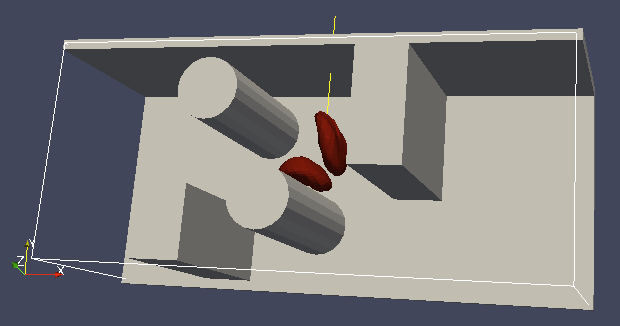
\includegraphics[width=4.2cm]{figures/2.png}     
    \end{center}
  \end{minipage}
  \hfill
  \begin{minipage}[t]{.32\textwidth}

      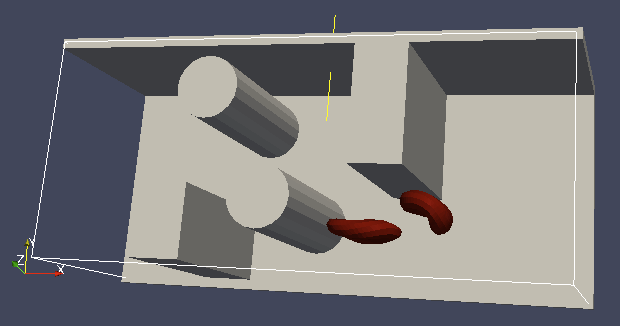
\includegraphics[width=4.2cm,left]{figures/3.png} 

  \end{minipage}
  \hfill
\end{figure} 

\section{Basic set up}

In order to be able to work with elastic objects, one needs to configure \es with the following options in myconfig.hpp:\\
\#define LB (or \#define LB\_GPU)\\
\#define LB\_BOUNDARIES (or \#define LB\_BOUNDARIES\_GPU)\\
\#define EXTERNAL\_FORCES\\
\#define MASS\\
\#define CONSTRAINTS\\
\#define VOLUME\_FORCE\\
\#define AREA\_FORCE\_GLOBAL\\
\#define SOFT\_SPHERE\\

To create an elastic object, we also need a triangulation of the surface of this object. Sample sphere and red blood cell are provided in the directory scripts/input. User can create her own in gmsh, salome or any other meshing software. The required format is as follows:\\

The file \verb|some_nodes.dat| should contain triplets of floats (one triplet per line), where each triplet represents the $x$, $y$ and $z$ coordinates of one node of the surface triangulation. No additional information should be written in this file, so this means that the number of lines equals the number of surface nodes. The coordinates of the nodes should be specified in such a way that the approximate center of mass of the object corresponds to the origin (0,0,0). This is for convenience when placing the objects at desired locations later.\\

The file \verb|some_triangles.dat| should also contain triplets of numbers, this time integers. These refer to the IDs of the nodes in the \verb|some_nodes.dat| file and specify which three nodes form a triangle together. Please, note that the nodes' IDs start at 0, i.e. the node written in the first line of \verb|some_nodes.dat| has ID 0, the node in the second line, has ID 1, etc.\\     

We can start our script by specifying these files:\\
\begin{tclcode}
  set fileNodes  "input/cell_nodes.dat"
  set fileTriangles "input/cell_triangles.dat"
\end{tclcode}
\vspace{0 mm}

And continue with setting up some molecular dynamics parameters of the simulation engine:\\
\begin{tclcode}
  setmd time_step 0.1    
  setmd skin 0.4
  thermostat off
\end{tclcode}
\vspace{0 mm}

The skin depth \verb|skin| is a parameter for the link--cell system, which tunes its performance, but will not be discussed here in detail. The one important thing a user needs to know about it is that it has to be strictly less than half the grid size.\\

Next we need to specify the simulation box:\\
\begin{tclcode}
  set boxX 50
  set boxY 22
  set boxZ 20
  setmd box_l $boxX $boxY $boxZ
\end{tclcode}
\vspace{0 mm}

Now comes the initialization of OIF module using\\ 
\begin{tclcode}
  oif_init
\end{tclcode}
\vspace{0 mm}

This command creates all the global variables and lists needed for templates and objects that will come afterwards. Elastic objects cannot be created directly. Each one has to correspond to a template that has been created first. The advantage of this approach is clear when creating many objects of the same type that only differ by e.g. position or rotation, because in such case it significantly speeds up the creation of objects that are just copies of the same template. The following command creates a template\\
\begin{tclcode}
  oif_create_template template-id 0 nodes-file $fileNodes \ 
  triangles-file $fileTriangles stretch 3.0 3.0 3.0 \
  ks 0.05 kb 0.01 kal 0.01 kag 0.01 kv 10.0
\end{tclcode}
\vspace{0 mm}

Each template has to have a unique ID specified using keyword \verb|template-id|. The IDs should start at 0 and increase consecutively. Another two mandatory arguments are \verb|nodes-file| and \verb|triangles-file| that specify data files with desired triangulation. All other arguments are optional: \verb|stretch| defines stretching in x, y, z direction and \verb|ks, kb, kal, kag, kv| specify the elastic properties of the object (stretching, bending, local area conservation, global area conservation, volume conservation respectively). The keywords can come in any order.\\

Once we have the template, we can start creating objects:\\
\begin{tclcode}
  oif_add_object object-id 0 template-id 0 origin 5 15 5 \
  rotate 0 0 [expr $pi/2] part-type 0 mass 1
  oif_add_object object-id 1 template-id 0 origin 5 5 15 \
  rotate 0 0 0 part-type 1 mass 1 
\end{tclcode} 
\vspace{0 mm}

Each object has to have a unique ID specified using keyword \verb|object-id|. The IDs should start at 0 and increase consecutively. Another three mandatory arguments are \verb|template-id|, \verb|origin| and \verb|part-type|. \verb|template-id| specifies which template will be used for this object. \verb|origin| gives placement of object's center in the simulation box. And \verb|part-type| assigns the particle type to all nodes of the given object. It is generally a good idea to specify a different \verb|part-type| for different objects since it can be then used to set up interactions among objects. The optional arguments are \verb|rotate| and \verb|mass|. Rotate takes three arguments - angles in radians - that determine how much the object is rotated around the x, y, z axes. (Note: if you want to use the variable  \verb|$pi|, you need to specify it beforehand, i.e. \verb|set pi 3.14159265359|). The optional keyword \verb|mass| takes one value and this mass will be assigned to each surface node of the object.\\

The interactions among objects are specified using\\   
\begin{tclcode}
  inter 0 1 soft-sphere 0.005 2.0 0.3 0.0
\end{tclcode}
\vspace{0 mm} 

where after \verb|inter| come the particle types of the two objects and \verb|soft-sphere| with four parameters stands for the "bouncy" interactions between the objects, once they come sufficiently close. (There are also other interaction types available in \es.) Similar interaction is defined with the boundaries:\\
\begin{tclcode}
 inter 0 10 soft-sphere 0.0001 1.2 0.1 0.0
 inter 1 10 soft-sphere 0.0001 1.2 0.1 0.0
\end{tclcode}  
\vspace{0 mm}

Here 10 (the second number after keyword \verb|inter|) is the the type of all boundaries and obstacles.

Finally, we specify the fluid, either by\\
\begin{tclcode}
 lbfluid grid 1 dens 1.0 visc 1.5 tau 0.1 friction 0.5
\end{tclcode}
\vspace{0 mm}

or\\ 
 \begin{tclcode}
 lbfluid gpu grid 1 dens 1.0 visc 1.5 tau 0.1 friction 0.5
\end{tclcode}
\vspace{0 mm}

depending on the available computational resources. (The GPU computation can be two orders of magnitude faster than the CPU.)\\

And finally we define the walls and boundaries. For clarity, these have been placed in a separate file \verb|boundaries.tcl|, which we'll go over in the next subsection. The source code of this boundaries script is included using the command\\
\begin{tclcode}
  source boundaries.tcl
\end{tclcode}
\vspace{0 mm}

but note, that the boundaries could have been specified directly at this point.\\  

\subsection*{Specification of boundaries}
As was previously mentioned, all the boundaries and obstacles are conveniently grouped in separate file \verb|boundaries.tcl|. Here we only go over rhomboids and cylinders, but note that other boundary types are available in \es.\\

The rhomboid is a 3D structure specified by one corner and three vectors originating from this corner. It can be a box and in that case the three vectors give the length, width and height. However, there is no requirement that the vectors are perpendicular (to each other or to the walls). It is a standard \es command.\\

Cylinder is specified by its center, radius, normal vector, and length. The length is the distance from center to either base, therefore it is only half the total "height". Note: the vtk-output is only available for cylinders with (0,0,1) normal, for now. \\ 

\begin{figure}[htbp]
  \hfill
  \begin{minipage}[t]{.22\textwidth}
      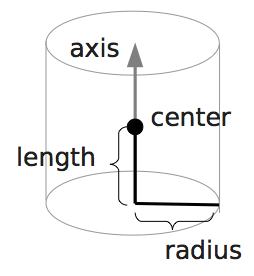
\includegraphics[width=2.3cm,right]{figures/cylinder.png}
	%\caption{Cylinder dimensions}
  \end{minipage}
  \hfill
  \begin{minipage}[t]{.45\textwidth}
   \begin{center}  
      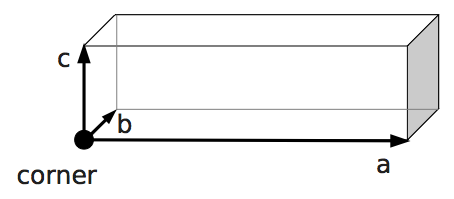
\includegraphics[width=5.2cm]{figures/rhomboid.png}     
      %\caption{Rhomboid dimensions}
    \end{center}
  \end{minipage}
  \hfill
  \begin{minipage}[t]{.3\textwidth}
      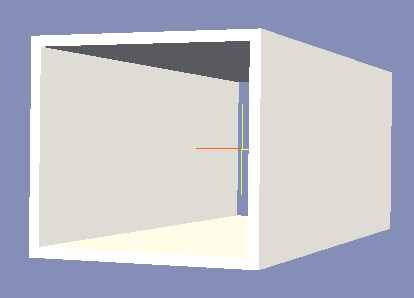
\includegraphics[width=4cm,left]{figures/channel.png} 
	%\caption{Channel geometry}
  \end{minipage}
  \hfill
\end{figure} 

Each wall and obstacle has to be specified separately as a fluid boundary and as a particle constraint. The former enters the simulation as a boundary condition for the fluid, the latter serves for particle-boundary interactions. Sample cylinder and rhomboid can then be defined as follows:\\
 \begin{tclcode}
# obstacle cylinder1 
set cX 16; set cY 17; set cZ 10;
set nX 0; set nY 0; set nZ 1;
set L 9
set r 3
set cylFile "output/cylinder1.vtk"
set n 20
output_vtk_cylinder $cX $cY $cZ $nX $nY $nZ $r $L $n $cylFile
constraint cylinder center $cX $cY $cZ axis $nX $nY $nZ radius $r \
length $L direction 1 type 10 
lbboundary cylinder center $cX $cY $cZ axis $nX $nY $nZ radius $r \
length $L direction 1
 \end{tclcode}
\vspace{0 mm}

 \begin{tclcode}
# obstacle rhomboid1
set corX 25; set corY 1; set corZ 1;
set aX 5; set aY 0; set aZ 0;
set bX 0; set bY 20; set bZ 0;
set cX 0; set cY 0; set cZ 10;
set rhomFile "output/rhomboid1.vtk"
output_vtk_rhomboid $corX $corY $corZ $aX $aY $aZ $bX $bY $bZ \
$cX $cY $cZ $rhomFile 
constraint rhomboid corner $corX $corY $corZ a $aX $aY $aZ b $bX $bY $bZ \
c $cX $cY $cZ direction 1 type 10 
lbboundary rhomboid corner $corX $corY $corZ a $aX $aY $aZ b $bX $bY $bZ \
c $cX $cY $cZ direction 1
 \end{tclcode}
 \vspace{0 mm}

Note that the cylinder also has an input parameter \verb|n|. This specifies number of rectangular faces on the side. The \verb|direction 1| determines that the fluid is on the "outside".\\
   
To create a rectangular channel, there are two possibilities. Either the walls are specified as the \verb|lbboundary wall| and \verb|constraint wall| with normal and distance from origin. Alternatively, the channel can be built using four flat rhomboids as can be seen in the picture above.\\  

Another way how to work with boundaries, is to set them up using \verb|lbboundary| and \verb|constraint|, make sure each boundary has a different type (the object-boundary interactions have to be modified accordingly) and then following command can be used for output of all of them at once:\\
 \begin{tclcode}
lbfluid print vtk boundary "boundary.vtk"
 \end{tclcode}
 \vspace{0 mm}
 
The differences in visualization in these two approaches are discussed later in this tutorial.

\section{Running the simulation}
One last thing needed before we can proceed to the main part of the simulation code, is to get the fluid moving. This can be done by setting the velocity of the individual \verb|lbnodes| on one side of the channel and letting the flow develop, but this is not a very convenient setup because it has to be done at every integration step and the tcl-C communication slows down the computation. The alternative is to set up a wall/rhomboid with velocity. This does not mean that the physical boundary is moving, but rather that it transfers specified momentum onto the fluid. This can be done using the command\\
\begin{tclcode}
lbboundary rhomboid velocity 0.01 0 0 corner 0 1 1 a 1 1 1 \
b 0 [expr $boxY-1] 1 c 0 1 [expr $boxZ-1] direction 1 
 \end{tclcode}
 \vspace{0 mm}

Now we can integrate the system:\\
\begin{tclcode}
set steps 200
set counter 0
while { $counter<150} {
    set cycle [expr $counter*$steps]
    puts "cycle $cycle" 
    integrate $steps
    incr counter
}
 \end{tclcode}
 \vspace{0 mm}
 
The script will print out a cycle number every 200 MD steps.
 
\section{Writing out data}

We have already discussed how to output the walls and obstacles for later visualization, but we also need output for fluid and objects. The fluid output is done using the standard \es command\\ 
\begin{tclcode}
 lbfluid print vtk velocity "output/fluid$cycle.vtk" 
 \end{tclcode}
 \vspace{0 mm}
 
 and one of the options for for object output is\\ 
 \begin{tclcode}
  oif_object_output object-id 0 vtk-pos "output/output_file.vtk"
  \end{tclcode}
  \vspace{0 mm}
  
This will save the positions of all surface nodes into the .vtk output file. The modified integration loop now looks like this:\\
\begin{tclcode}
while { $counter<150} {
    set cycle [expr $counter*$steps]
    puts "cycle $cycle" 
    lbfluid print vtk velocity "output/fluid$cycle.vtk" 
    oif_object_output object-id 0 vtk-pos "output/cell0_$cycle.vtk"
    oif_object_output object-id 1 vtk-pos "output/cell1_$cycle.vtk"
    integrate $steps
    incr counter
}
 \end{tclcode}
 \vspace{0 mm}
 
 where each object has its own output file and a new file is written every \verb|$steps| steps.

\section{Visualization}
For visualization we suggest the free software Paraview. All .vtk files (boundaries, fluid, objects at all time steps) can be loaded at the same time. The loading is a two step process, because only after pressing the Apply button, are the files actually imported. Using the eye icon to the left of file names, one can turn on and off the individual objects and/or boundaries. It is also possible to do this when one imports all the boundaries from a single .vtk file (created using command \verb|lbfluid print vtk| \verb|boundary| \verb|"boundary.vtk"|), however only when each boundary had been assigned a unique type number and is then selected in the bottom left menu by this number.\\ 

Fluid can be visualized using Filters/Alphabetical/Glyph (or other options from this menu. Please, refer to the Paraview user's guide for more details).\\

Note, that Paraview does not automatically reload the data if they have been changed in the input folder, but a useful thing to know is that the created filters can be "recycled". Once you delete the old data, load the new data and right-click on the existing filters, you can re-attach them to the new data.\\
  
It is a good idea to output and visualize the boundaries and objects just prior to running the actual simulation, to make sure that the geometry is correct and no objects intersect with any boundaries. This would cause "particle out of range" error and crash the simulation.\\ 

\section{Other available OIF commands}

The OIF commands that we have covered so far are\\
 \begin{tclcode}
oif_init
oif_create_template
oif_add_object
oif_object_output
 \end{tclcode}
 \vspace{0 mm}
 
Other available OIF commands are\\
\begin{tclcode}
oif_info
oif_mesh_analyze
oif_object_analyze
oif_object_set
\end{tclcode}
 \vspace{0 mm}

and there are more still being added. Details about all the OIF commands can be found in the official \es User Guide and at our website\\ http://cell-in-fluid.fri.uniza.sk/sites/default/files/document/oif\_documentation.pdf\\ 
And we would be pleased to hear from you about any suggestions on further functionality and improvements.

\end{document}
